% Lezione del 15/03/2021

\documentclass[../main.tex]{subfiles}

\begin{document}

\chapter{Introduzione}
Le \textbf{istruzioni} sono dei comandi nella "lingua del computer"
\begin{itemize}
    \item \textbf{linguaggio Assembly}: formato di istruzioni comprensibili all'uomo
    \item \textbf{linguaggio macchina}: formato di istruzioni comprensibili dal computer (0 e 1)
\end{itemize}

\section{Principi base}
Principi base della progettazione dell'architettura MIPS:
\begin{enumerate}
    \item la semplicità favorisce la regolarità
    \item bisogna cercare di rendere il caso più comune il caso più veloce
    \item tutto ciò che è piccolo è più veloce
    \item un buon progetto richiede un buon compromesso
\end{enumerate}

\subsection*{Principio base - \Large Primo}
``\textit{La semplicità favorisce la regolarità.}"
\begin{itemize}
    \item formato delle istruzioni consistente
    \item stesso numero di operandi (due sorgenti ed uno destinazione)
    \item più facile da decodificare e gestire in hardware
\end{itemize}

\subsection*{Principio base - \Large Secondo}
``\textit{Bisogna cercare di rendere il caso più comune il caso più veloce.}"
\\[2mm] Lo scopo del MIPS è di avere una CPU di tipo
RISC\hspace*{.25mm}\footnote{\hspace*{.5mm}RISC:
Reduced Instruction Set Computer}
(in contrapposizione alle altre architetture, di tipo
CISC\hspace*{.25mm}\footnote{\hspace*{.5mm}CISC:
Complex Instruction Set Computers})
con un numero ridotto di istruzioni (solo quelle più comuni)
permettendo di eseguire più velocemente i casi più frequenti.

\subsection*{Principio base - \Large Terzo}
``\textit{Tutto ciò che è piccolo è più veloce.}"
\\[2mm] I RISC, poiché risparmiano spazio e unità di controllo, tendono a
dedicare lo spazio disponibile per aumentare il numero dei registri
(rispetto ai processori di tipo CISC).
\\ MIPS ha un numero limitato di registri.
\\[3mm]
\underline{\textbf{Nota bene}: Se avesse molti registri sarebbe più complicato decodificare il numero
dei registri.}

\subsection*{Principio base - \Large Quarto}
``\textit{Più facile da decodificare e gestire in hardware.}"
\\[2mm] Esistono certe istruzioni che utilizzano 2 oppure 3 registri (es. \texttt{lw,sw} ne usano 2, \texttt{add,sub} ne usano 3).
\\ Purtroppo non posso avere una regolarità totale; quindi, cerco di trovare il miglior compromesso.
\\[3mm]
\underline{Per garantire i principi 1 e 3, cerco di avere il minor numero di formati possibili.}

\newpage

\section{Istruzioni}
Qui di seguito sono presenti alcuni esempi
di utilizzo delle istruzioni MIPS.
\subsection{Addizione e sottrazione algebrica}
La \texttt{add} (\textit{somma}) e la \texttt{sub}
(\textit{differenza}) sono mnemonici
\hspace*{.25mm}\footnote{\hspace*{.5mm}Mnemonico:
il nome di un istruzione.} che mi specificano
il tipo di operazione da eseguire.
\\[3mm]
\begin{tabular}{ p{1mm} p{2.5cm} p{2.5cm} p{1cm} | p{1cm} p{2.5cm} p{2.5cm} p{1mm} }
    & \underline{\textbf{Addizione}} & & & & \underline{\textbf{Sottrazione}} & \vspace*{1cm} \\
    \hline
    \rule{0pt}{1.5\normalbaselineskip} &

    \multirow{2}{*}{\textbf{Codice C}} & \textbf{Codice MIPS \newline assembly} & & & \multirow{2}{*}{\textbf{Codice C}} & \textbf{Codice MIPS \newline assembly} & \\
    & \texttt{a = b + c} & \texttt{add a, b, c} & & & \texttt{a = b - c} & \texttt{sub a, b, c} & \\

    \\
\end{tabular}
\\[1.5mm]
Operandi:
\begin{itemize}
    \item \texttt{a}: operando destinazione (dove scrive il risultato della somma)
    \item \texttt{b,c}: operandi sorgenti (gli addendi da sommare)
\end{itemize}

\subsection{Istruzioni multiple}
Se ho da gestire più variabili devo utilizzare una variabile temporanea.
\\[3mm]
\begin{tabular}{ p{7cm} p{7cm} }
    \textbf{Codice C} & \textbf{Codice MIPS assembly} \\
    \multirow{2}{*}{\texttt{a = b + c - d;}} & \texttt{add t, b, c \hspace*{2mm} \# t = b + c} \\
	& \texttt{sub a, t, d \hspace*{2mm} \# a = t - d} \\
\end{tabular}
\\[3mm]
\underline{\textbf{Nota bene:} il carattere '\#' serve per iniziare un commento.}

\subsection{Istruzioni con registri}
I registri tornano molto utili nelle istruzioni.
\\[3mm]
\begin{tabular}{ p{7cm} p{7cm} }
    \textbf{Codice C} & \textbf{Codice MIPS assembly} \\
    \multirow{2}{*}{\texttt{a = b + c}} & \texttt{\# \$s0 = a, \$s1 = b, \$s2 = c} \\
	& \texttt{add \$s0, \$s1, \$s2} \\
\end{tabular}

\subsection{Istruzioni con costanti}
La \texttt{addi} (add immediate) è un mnemonico che mi permette di sommare
una costante. \\
Si dedicano \textbf{16 bit} per la rappresentazione
delle costanti e si sommano in \textbf{complemento a due}. \\
\\[3mm]
\begin{tabular}{ p{7cm} p{7cm} }
    \textbf{Codice C} & \textbf{Codice MIPS assembly} \\
    \multirow{3}{*}{\makecell{\hspace*{-2mm}\texttt{a = a + 4;} \\ \texttt{b = a - 12;}}} & \texttt{\# \$s0 = a, \$s1 = b} \\
	& \texttt{addi \$s0, \$s0, 4} \\
    & \texttt{addi \$s1, \$s0, -12} \\
\end{tabular}
\\[3mm]
\underline{\textbf{Nota bene:} non è necessario definire nell'insieme
di istruzioni la \texttt{subi} in quanto
basta aggiungere}
\newline
\underline{un segno negativo nella
\texttt{addi} (risparmio un'istruzione).}

\newpage

\section{Operandi}
Gli operandi possono essere:
\begin{itemize}
    \item registri
    \item memorie
    \item costanti (alternativamente chiamati "\textbf{valori immediati}")
\end{itemize}

\subsection{Registri}
In MIPS si hanno 32 registri organizzati su 32 bit (quindi è
un'architettura da 32 bit). \\
Quindi, si definisce il parallelismo di una CPU come il numero di bit
dei \textbf{registri interni}. \\
Questa è la dimensione massima dei dati (in termini
di bit/byte) che possono essere trasferiti \\ da memoria
a CPU e viceversa.
\\[1mm]
\underline{Non e' dunque legato al numero di registri, ma al numero di bit dei
registri interni (nel MIPS questi} \\ \underline{due numeri sono sempre 32).}
\\[3mm]
Nella tabella seguente (Tabella 1.1) sono elencati i registri utilizzati da MIPS.
\begin{table}[htb!]
    \centering
    
    \setlength{\tabcolsep}{12pt}
    \renewcommand{\arraystretch}{1.5}
    \definecolor{ccolor}{rgb}{0.67, 0.9, 0.93}
    \begin{tabular}{ V{4} p{2cm} | p{4cm} | p{5cm} V{4}}
        \hlineB{4}
        \rowcolor{ccolor}
        { \textbf{Nome} } & { \textbf{Numero di registro} } & { \textbf{Utilizzo} } \\
        \hlineB{4}
        \texttt{\$0} & 0 & valore costante 0 \\
        \hline
        \texttt{\$at} & 1 & assembler temporary \\
        \hline
        \texttt{\$v0-\$v1} & 2 - 3 & valori di ritorno \\
        \hline
        \texttt{\$a0-\$a3} & 4 - 7 & argomenti \\
        \hline
        \texttt{\$t0-\$t7} & 8 - 15 & temporanei \\
        \hline
        \texttt{\$s0-\$s7} & 16 - 23 & variabili salvate \\
        \hline
        \texttt{\$t8-\$t9} & 24 - 25 & "molto" temporanei \\
        \hline
        \texttt{\$k0-\$k1} & 26 - 27 & temporanei per il SO \\
        \hline
        \texttt{\$gp} & 28 & puntatore globale \\
        \hline
        \texttt{\$sp} & 29 & puntatore dello stack \\
        \hline
        \texttt{\$fp} & 30 & puntatore della finestra \\
        \hline
        \texttt{\$ra} & 31 & indirizzo di ritorno \\
        \hlineB{4}
    \end{tabular}
    \caption{Insieme dei registri MIPS}
\end{table}

\noindent
\underline{\textbf{Nota bene}: i registri sono più veloci della memoria.}

\newpage

\subsection{Memorie}
\underline{Le memorie sono necessarie in quanto non sono sufficienti
32 registri per memorizzare i dati.}
\\[3mm] La memoria ha una dimensione maggiore rispetto ai registri
ma lavora con velocità ridotta.
\\[1mm] \textit{Una buona prassi è quella di mantenere nei registri le variabili utilizzate
più frequentemente e limitarsi ad usare la memoria il meno possibile.}
\subsubsection*{Organizzazione della memoria}
La memoria ha degli indirizzi che fanno riferimento ad un singolo byte.
\hspace*{-.5mm}Tuttavia, in MIPS, i dati\\hanno un'organizzazione su 32 bit,
quindi sono organizzati in word (indirizzi distanti di 4 byte).
\\Si può indirizzare la memoria associata a MIPS come singoli byte.
\begin{table}[htb!]
    \centering

    \setlength{\tabcolsep}{18pt}
    \begin{tabular}{ c | c | c}
        \multicolumn{1}{c}{\textbf{Indirizzi}} & \multicolumn{1}{c}{\textbf{Dati}} \\
        \vdots & \vdots & \vdots \\
        \cline{2-2}
        \texttt{0000000C} & \texttt{4 0 F 3 0 7 8 8} & \texttt{Word 3} \\
        \cline{2-2}
        \texttt{00000008} & \texttt{0 1 E E 2 8 4 2} & \texttt{Word 2} \\
        \cline{2-2}
        \texttt{00000004} & \texttt{F 2 F 1 A C 0 7} & \texttt{Word 1} \\
        \cline{2-2}
        \texttt{00000000} & \texttt{A B C D E F 7 8} & \texttt{Word 0} \\
        \cline{2-2}
    \end{tabular}
\end{table}

\subsubsection*{Lettura della memoria}
\underline{\textbf{Word}}
\begin{table}[htb!]
    \centering
    \begin{tabular}{ p{4.5cm} | p{10.5cm} }
        Nome & Valore \\
        \hline
        Istruzione (mnemonico) & \texttt{lw (load word)} \\
        Formato & \texttt{lw <valore salvato>, <offset>(<indirizzo base>)}
    \end{tabular}
\end{table}
\newline
\underline{\textbf{Byte}}
\begin{table}[htb!]
    \centering
    \begin{tabular}{ p{4.5cm} | p{10.5cm} }
        Nome & Valore \\
        \hline
        Istruzione (mnemonico) & \texttt{lb (load byte)} \\
    \end{tabular}
\end{table}
\newline
Per calcolare l'indirizzo in memoria devo fare la somma tra
l'indirizzo base, che è contenuto in un registro, e un offset
che è una costante.
\\[3mm]
\textbf{Esempio} \\
Caricare una word di dati nell'indirizzo di
memoria 4 dentro \texttt{\$s3} (\texttt{\$s3}
contiene il valore \texttt{0xF2F1AC07} dopo
il caricamento).
\\[3mm]
\begin{tabular}{ l }
    \textbf{Codice MIPS assembly} \\
    \texttt{lw \$s3, 4(\$0) \hspace*{2mm} \# legge la word all'indirizzo 4 dentro \$s3}
\end{tabular}
\\[3mm]

\begin{table}[htb!]
    \centering

    \setlength{\tabcolsep}{6pt}
    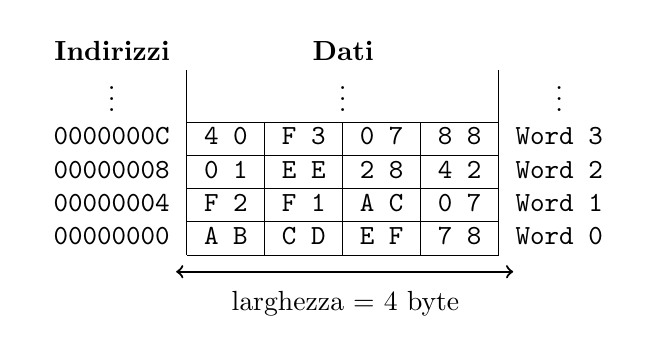
\begin{tikzpicture}
        \node(table) {
            \begin{tabular}{ c | c | c | c | c | c}
                \multicolumn{1}{c}{\textbf{Indirizzi}} & \multicolumn{4}{c}{\textbf{Dati}} \\
                \vdots & \multicolumn{4}{ c | }{\vdots} & \vdots \\
                \cline{2-5}
                \texttt{0000000C} & \texttt{4 0} & \texttt{F 3} & \texttt{0 7} & \texttt{8 8} & \texttt{Word 3} \\
                \cline{2-5}
                \texttt{00000008} & \texttt{0 1} & \texttt{E E} & \texttt{2 8} & \texttt{4 2} & \texttt{Word 2} \\
                \cline{2-5}
                \texttt{00000004} & \texttt{F 2} & \texttt{F 1} & \texttt{A C} & \texttt{0 7} & \texttt{Word 1} \\
                \cline{2-5}
                \texttt{00000000} & \texttt{A B} & \texttt{C D} & \texttt{E F} & \texttt{7 8} & \texttt{Word 0} \\
                \cline{2-5}
            \end{tabular}
        };

        \draw [<->, thick]
            (-1.93,-1.6) -- (2.35,-1.6);

        \node[text width=4cm, align=center] at (.22,-2) {larghezza = 4 byte};

    \end{tikzpicture}
\end{table}

\newpage

\subsubsection*{Scrittura della memoria}
\underline{\textbf{Word}}
\begin{table}[htb!]
    \centering
    \begin{tabular}{ p{4.5cm} | p{10.5cm} }
        Nome & Valore \\
        \hline
        Istruzione (mnemonico) & \texttt{sw (store word)} \\
        Formato & \texttt{sw <valore caricato>, <offset>(<indirizzo base>)}
    \end{tabular}
\end{table}
\newline
\underline{\textbf{Byte}}
\begin{table}[htb!]
    \centering
    \begin{tabular}{ p{4.5cm} | p{10.5cm} }
        Nome & Valore \\
        \hline
        Istruzione (mnemonico) & \texttt{sb (store byte)} \\
    \end{tabular}
\end{table}
\\[3mm]
\textbf{Esempio} \\
Scrivere il valore di \texttt{\$t4} nell'indirizzo di memoria 8.
\\[3mm]
\begin{tabular}{ l }
    \textbf{Codice MIPS assembly} \\
    \texttt{sw \$t4, 0x8(\$0) \hspace*{2mm} \# scrive il valore in \$t4 all'indirizzo di memoria 8}
\end{tabular}
\\[3mm]

\begin{table}[htb!]
    \centering

    \setlength{\tabcolsep}{6pt}
    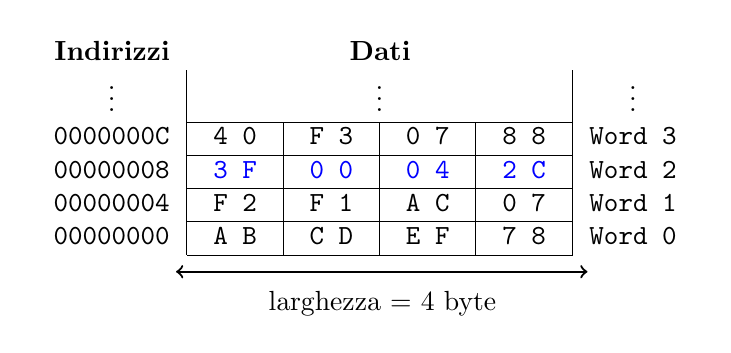
\begin{tikzpicture}
        \node(table) {
            \begin{tabular}{ c | c | c | c | c | c}
                \multicolumn{1}{c}{\textbf{Indirizzi}} & \multicolumn{4}{c}{\textbf{Dati}} \\
                \vdots & \multicolumn{4}{ c | }{\vdots} & \vdots \\
                \cline{2-5}
                \texttt{0000000C} & \texttt{4 0} & \texttt{F 3} & \texttt{0 7} & \texttt{8 8} & \texttt{Word 3} \\
                \cline{2-5}
                \texttt{00000008} & { \color{blue} \textbf{\texttt{3 F}} } & { \color{blue} \textbf{\texttt{0 0}} } & { \color{blue} \textbf{\texttt{0 4}} } & { \color{blue} \textbf{\texttt{2 C}} } & \texttt{Word 2} \\
                \cline{2-5}
                \texttt{00000004} & \texttt{F 2} & \texttt{F 1} & \texttt{A C} & \texttt{0 7} & \texttt{Word 1} \\
                \cline{2-5}
                \texttt{00000000} & \texttt{A B} & \texttt{C D} & \texttt{E F} & \texttt{7 8} & \texttt{Word 0} \\
                \cline{2-5}
            \end{tabular}
        };

        \draw [<->, thick]
            (-2.4,-1.6) -- (2.825,-1.6);

        \node[text width=5cm, align=center] at (.22,-2) {larghezza = 4 byte};

    \end{tikzpicture}
\end{table}
\noindent
\underline{\textbf{Nota bene}: l'offset può essere scritto
in decimale o in esadecimale.}

\newpage

\subsubsection*{Little e Big Endian}
Ci sono due tecniche per salvare una \texttt{word} in memoria:
\begin{itemize}
    \item little endian: \hspace*{.5cm} inizia dal byte meno significativo
    \item big endian: \hspace*{.755cm} inizia dal byte più significativo
\end{itemize}

\vspace*{3mm}
\noindent
\textbf{Esempio} \\
Si supponga che il registro \texttt{\$t0} inizialmente
contenga il valore \texttt{0x23456789}.
\\[2mm] Se il codice viene eseguito su un sistema big endian,
qual'è il valore di \texttt{\$s0}? \\
In un sistema little endian?
\\[2mm]
\hspace*{6mm} \texttt{sw \$t0, 0(\$0)} \\
\hspace*{6mm} \texttt{lb \$s0, 1(\$0)}
\\[-2mm]

\begin{table}[htb!]
    \centering

    \begin{minipage}{.15\linewidth}
        \centering

        \setlength{\tabcolsep}{6pt}
        \renewcommand{\arraystretch}{1.5}
        \definecolor{ccolor}{rgb}{0.67, 0.9, 0.93}
        \caption*{}
        \begin{tabular}{ r }
            Indirizzo byte \\
            Valore dato
        \end{tabular}
        \caption*{}
    \end{minipage}
    \begin{minipage}{.2\linewidth}
        \centering

        \setlength{\tabcolsep}{6pt}
        \renewcommand{\arraystretch}{1.5}
        \definecolor{ccolor}{rgb}{0.67, 0.9, 0.93}
        \caption*{\textbf{Big Endian}}
        \begin{tabular}{ | c | c | c | c | }
            \\[-9mm]
            \multicolumn{1}{ c }{\multirow{2}{*}{0}} &
            \multicolumn{1}{ c }{\multirow{2}{*}{1}} &
            \multicolumn{1}{ c }{\multirow{2}{*}{2}} &
            \multicolumn{1}{ c }{\multirow{2}{*}{3}} \\[-6.5mm]
            & & & \\[3.25mm]
            \hline
            23 & 45 & 67 & 89 \\
            \hline
        \end{tabular}
        \caption*{MSB \hspace*{1.5cm} LSB}
    \end{minipage}
    \begin{minipage}{.15\linewidth}
        \centering

        \setlength{\tabcolsep}{6pt}
        \renewcommand{\arraystretch}{1.5}
        \definecolor{ccolor}{rgb}{0.67, 0.9, 0.93}
        \caption*{}
        \begin{tabular}{ c }
            \large Address \\
            0 \\
        \end{tabular}
        \caption*{}
    \end{minipage}
    \begin{minipage}{.2\linewidth}
        \centering

        \setlength{\tabcolsep}{6pt}
        \renewcommand{\arraystretch}{1.5}
        \definecolor{ccolor}{rgb}{0.67, 0.9, 0.93}
        \caption*{\textbf{Little Endian}}
        \begin{tabular}{ | c | c | c | c | }
            \\[-9mm]
            \multicolumn{1}{ c }{\multirow{2}{*}{3}} &
            \multicolumn{1}{ c }{\multirow{2}{*}{2}} &
            \multicolumn{1}{ c }{\multirow{2}{*}{1}} &
            \multicolumn{1}{ c }{\multirow{2}{*}{0}} \\[-6.5mm]
            & & & \\[3.25mm]
            \hline
            23 & 45 & 67 & 89 \\
            \hline
        \end{tabular}
        \caption*{MSB \hspace*{1.5cm} LSB}
    \end{minipage}
    \begin{minipage}{.15\linewidth}
        \centering

        \setlength{\tabcolsep}{6pt}
        \renewcommand{\arraystretch}{1.5}
        \definecolor{ccolor}{rgb}{0.67, 0.9, 0.93}
        \caption*{}
        \begin{tabular}{ l }
            Indirizzo byte \\
            Valore dato
        \end{tabular}
        \caption*{}
    \end{minipage}
\end{table}

\begin{table}[htb!]
    \centering

    \begin{minipage}{.2\linewidth}
        \centering

        \begin{tabular}{ | c | }
            Risultato \\
            \texttt{0x00000045} \\
        \end{tabular}
    \end{minipage}
    \begin{minipage}{.15\linewidth}
        \centering
        \hspace*{0cm}
    \end{minipage}
    \begin{minipage}{.2\linewidth}
        \centering

        \begin{tabular}{ | c | }
            Risultato \\
            \texttt{0x00000067} \\
        \end{tabular}
    \end{minipage}
\end{table}

\subsubsection*{Allineamento dei dati}
\underline{Nella lettura e scrittura di una word, gli
indirizzi devono essere multipli di 4.}
\\[2mm]
Per esempio, questa istruzione \\
\hspace*{6mm} \texttt{lw \$s0, 7(\$0)} \\
non ha senso, in quanto andrebbe a leggere
una word all'indirizzo 7 (non è multiplo di 4).
\\[1mm]
Si può scegliere la posizione del mio codice/dati utilizzando la direttiva
(pseudoistruzione) \texttt{.align}
altrimenti il codice è allineato in automatico dal compilatore.
\\[1mm]
\underline{\textbf{Nota bene}: la dimensione di un'istruzione è di 32 bit.} \\

\begin{table}[htb!]
    \centering

    \setlength{\tabcolsep}{12pt}
    \renewcommand{\arraystretch}{1.5}
    \definecolor{ccolor}{rgb}{0.67, 0.9, 0.93}
    \begin{tabular}{ V{4} c | c | c V{4} }
        \hlineB{4}
        \rowcolor{ccolor}
        \textbf{Dato} & \textbf{Dimensione (byte)} & \textbf{Da salvare nell'indirizzo} \\
        \hlineB{4}
        byte & $\text{1 = 2}^\text{0}$ & Qualunque \\
        \hline
        \nicefrac{1}{2} word & $\text{2 = 2}^\text{1}$ & Multiplo di 2 \\
        \hline
        word & $\text{4 = 2}^\text{2}$ & Multiplo di 4 \\
        \hline
        double & $\text{8 = 2}^\text{3}$ & Multiplo di 8 \\
        \hlineB{4}
    \end{tabular}
\end{table}
\noindent
\textbf{Esempio}
\\ Esempio di allineamento di un tipo di dato \texttt{word} in memoria.
\begin{table}[htb!]
    \begin{minipage}{.5\linewidth}
        \centering

        \setlength{\tabcolsep}{12pt}
        \renewcommand{\arraystretch}{2}
        \definecolor{ccolor}{rgb}{0.67, 0.9, 0.93}
        \begin{tabular}{ V{2} p{.75cm} V{2} p{.75cm} V{2} p{.75cm} V{2} p{.75cm} V{2} }
            \multicolumn{4}{ V{2} c V{2} }{\textbf{\vdots}} \\
            \hlineB{2}
            \multicolumn{4}{ V{2} c V{2} }{} \\
            \hlineB{2}
            \cellcolor{brown!75} & & & \\
            \hlineB{2}
            & \cellcolor{brown!75} & \cellcolor{brown!75} & \cellcolor{brown!75} \\
            \hlineB{2}
            \multicolumn{4}{ V{2} c V{2} }{\textbf{\vdots}} \\
        \end{tabular}
        \caption*{\textbf{Allineamento errato}}
    \end{minipage}
    \begin{minipage}{.5\linewidth}
        \centering

        \setlength{\tabcolsep}{12pt}
        \renewcommand{\arraystretch}{2}
        \definecolor{ccolor}{rgb}{0.67, 0.9, 0.93}
        \begin{tabular}{ V{2} p{.75cm} V{2} p{.75cm} V{2} p{.75cm} V{2} p{.75cm} V{2} }
            \multicolumn{4}{ V{2} c V{2} }{\textbf{\vdots}} \\
            \hlineB{2}
            \multicolumn{4}{ V{2} c V{2} }{} \\
            \hlineB{2}
            \multicolumn{4}{ V{2} c V{2} }{} \\
            \hlineB{2}
            \cellcolor{brown!75} & \cellcolor{brown!75} & \cellcolor{brown!75} & \cellcolor{brown!75} \\
            \hlineB{2}
            \multicolumn{4}{ V{2} c V{2} }{\textbf{\vdots}} \\
        \end{tabular}
        \caption*{\textbf{Allineamento corretto}}
    \end{minipage}
\end{table}

\subsection{Costanti}
I valori immediati (o costanti) hanno l'esigenza di essere rappresentati
in questi due casi:
\begin{itemize}
    \item definizione di un eventuale offset
    \item inserimento di una costante all'interno
    di un'espressione numerica
\end{itemize}
\vspace*{2mm}
\underline{\textbf{Nota bene:} le costanti sono rappresentate da una codifica a 16 bit (in complemento
a due, per numeri} \\
\underline{positivi e negativi).}

\newpage

\end{document}